\documentclass[12pt]{article}

\usepackage{times,mathptmx}
\usepackage[pdftex]{graphicx}
\usepackage{pdflscape}
\usepackage{subcaption}
\usepackage{graphicx}
\usepackage{float}
\usepackage[section]{placeins}
\usepackage{fancyhdr}
\usepackage{enumitem}
\usepackage{xcolor}
\usepackage{listings}
\usepackage{textcomp}

\definecolor{lbcolor}{rgb}{0.96,0.96,0.96}
\lstset{
    backgroundcolor=\color{lbcolor},
    tabsize=4,
    rulecolor=,
    language=Fortran,
	basicstyle=\footnotesize \ttfamily,	
        upquote=true,
        aboveskip={\baselineskip},
        belowskip={\baselineskip},
        columns=fixed,
        extendedchars=true,
        breaklines=true,
        breakatwhitespace=true,
        frame=none,
        showtabs=false,
        showspaces=false,
        showstringspaces=false,
        identifierstyle=\ttfamily,
        keywordstyle=\color[rgb]{0,0,0},
        commentstyle=\color[rgb]{0,0,0},
        stringstyle=\color[rgb]{0,0,0},
}

\usepackage{tocloft}
\usepackage[nottoc,notlof,notlot]{tocbibind} % Put the bibliography and index in the ToC

\pagestyle{fancy}
\rhead{}
\lhead{}
\chead{}
\cfoot{Page \thepage}
%\renewcommand{\headrulewidth}{0.4pt}
\renewcommand{\footrulewidth}{0.4pt}

\usepackage{color}
\usepackage{amsmath}
\usepackage{multirow}
\definecolor{linknavy}{rgb}{0,0,0.50196}
\definecolor{linkred}{rgb}{1,0,0}
\definecolor{linkblue}{rgb}{0,0,1}

\usepackage{xr-hyper}
\usepackage[pdftex,
        colorlinks=true,
        urlcolor=linkblue,     % \href{...}{...} external (URL)
        citecolor=linkred,     % citation number colors
        linkcolor=linknavy,    % \ref{...} and \pageref{...}
        pdfproducer={pdflatex},
        pagebackref,
        pdfpagemode=UseNone,
        bookmarksopen=true,
        plainpages=false,
        verbose]{hyperref}

\setlength{\textwidth}{6.5in}
\setlength{\textheight}{9.0in}
\setlength{\topmargin}{0.in}
\setlength{\headheight}{0.in}
\setlength{\headsep}{0.1in}
\setlength{\parindent}{0.25in}
\setlength{\oddsidemargin}{0.0in}
\setlength{\evensidemargin}{0.0in}

\newcommand{\pp}{\prime\prime}

\begin{document}

\bibliographystyle{unsrt}
\thispagestyle{empty}

\begin{center}
{\bf\Large Guidelines for Participation in the MaCFP-4 Workshop} \\
{\large June, 2026\\La Rochelle, France}
\end{center}

\begin{figure}[h]
  \centering
  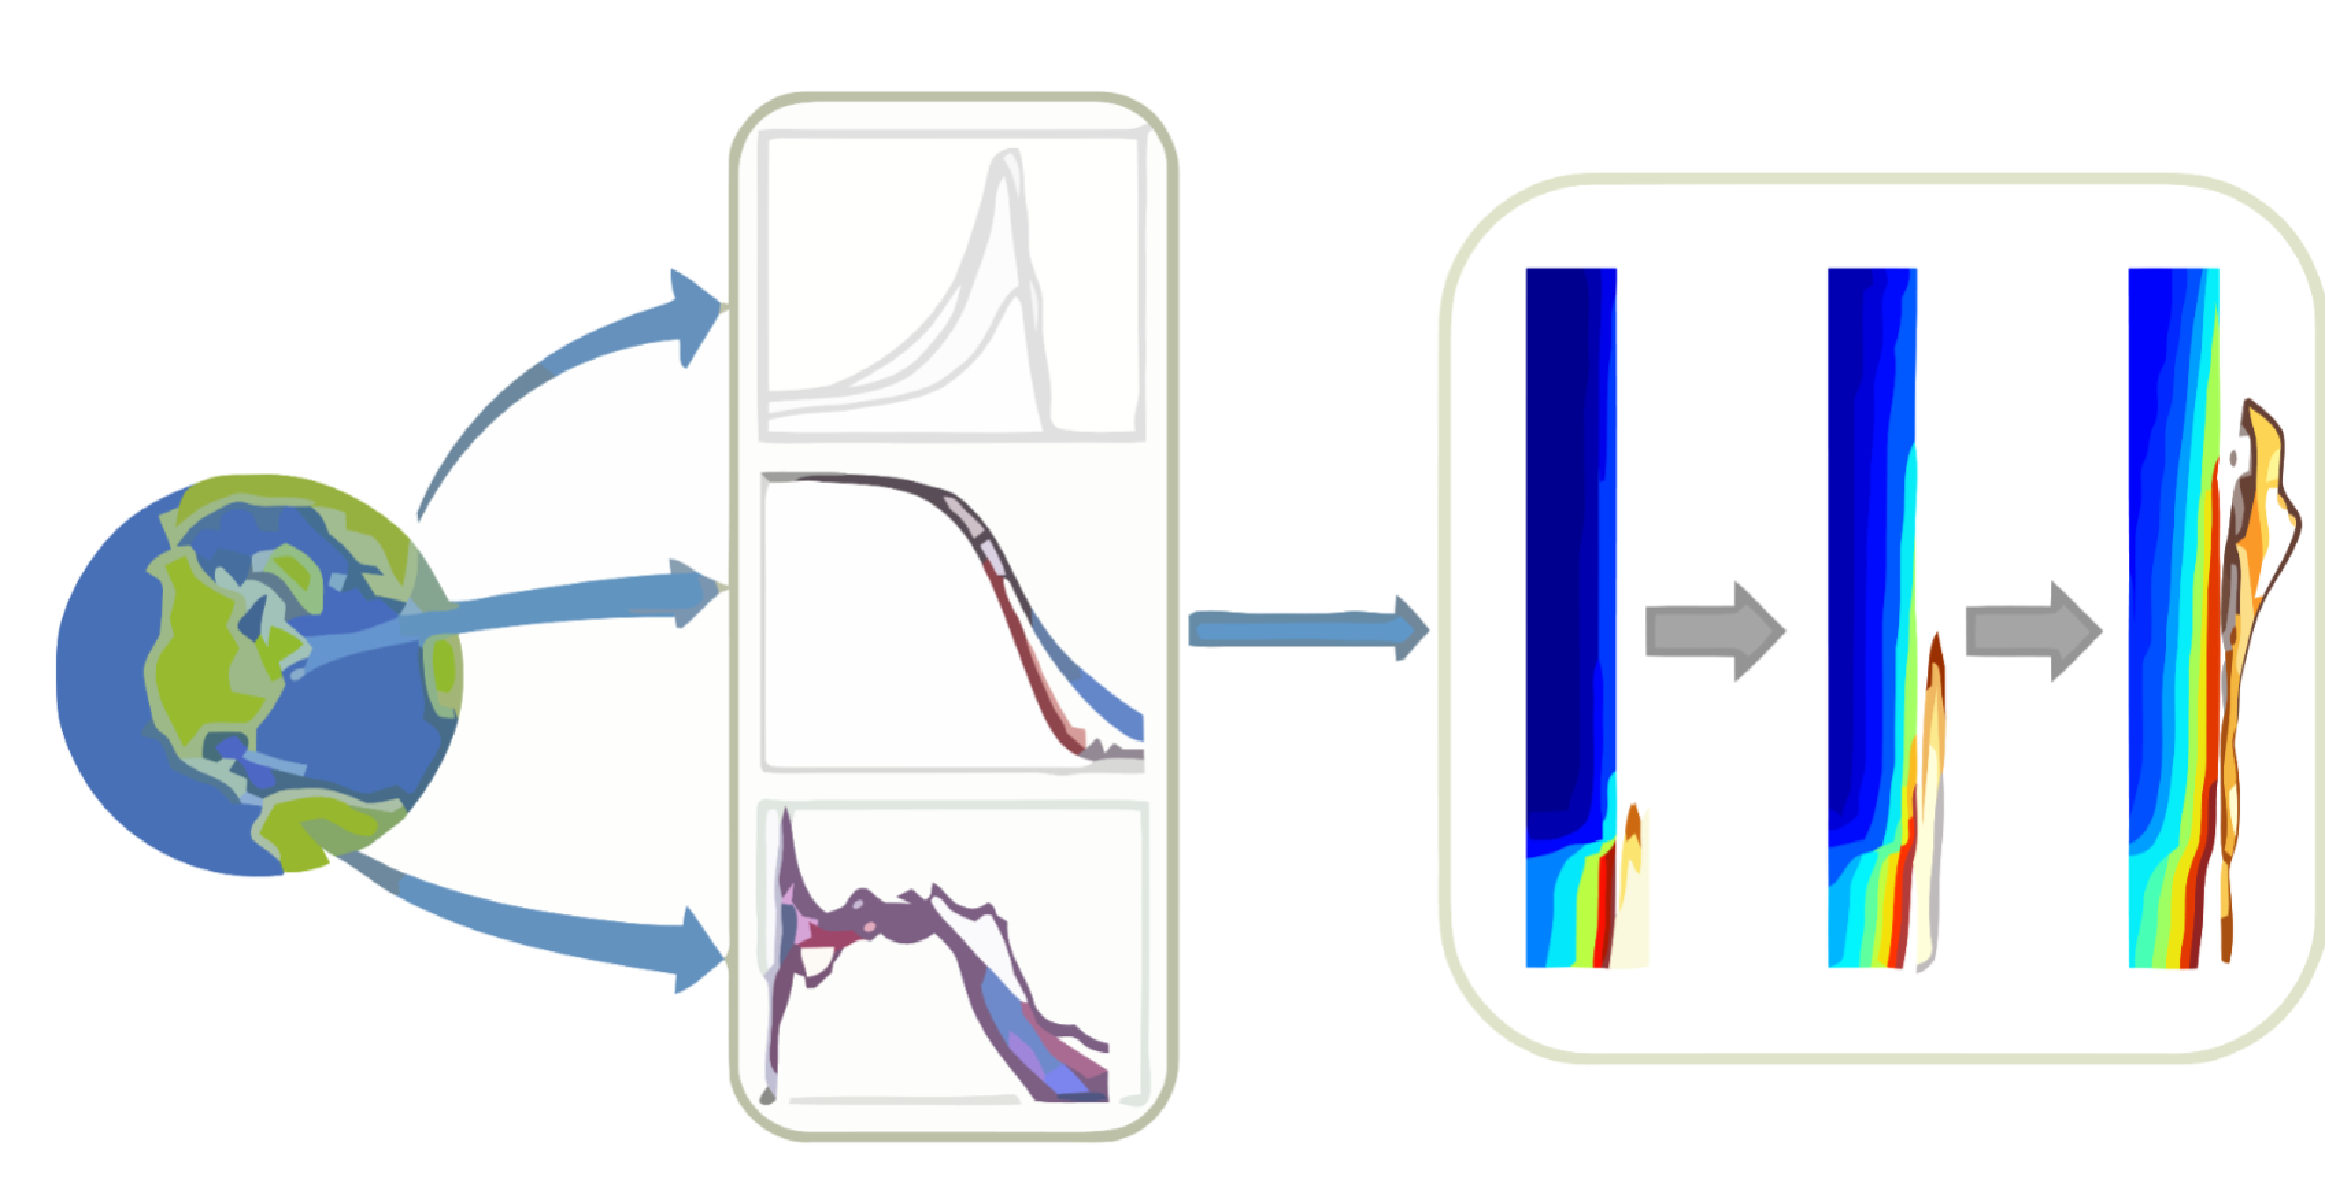
\includegraphics[width=6in]{../MaCFP_Logo.pdf}
  \label{Cover_Image}
\end{figure}

\vfill

\begin{minipage}{0.25\textwidth}
\begin{figure}[H]

\includegraphics[width=1.8in]{../IAFSSLogo.pdf}
\end{figure}
\end{minipage} \hfill
\begin{minipage}{0.65\textwidth}
\begin{flushright}
\begin{small}
{\bf The MaCFP Working Group Organizing Committee:} \\
{\footnotesize \underline{Condensed Phase Subgroup:} Benjamin Batiot (University of Poitiers, France); Morgan Bruns (St. Mary's University, USA); Simo Hostikka (Aalto University, Finland); Isaac Leventon (National Institute of Standards and Technology, USA); Yuji Nakamura (Toyohashi University of Technology, Japan); Pedro Reszka (Universidad Adolfo Ibáñez, Chile); Thomas Rogaume (University of Poitiers, France); Stanislav Stoliarov (University of Maryland, USA)}\\
{\footnotesize  \underline{Radiation Heat Transfer Subgroup:} Simo Hostikka (Aalto University, Finland) and Fabian Bränström (University of Wuppertal)}\\
{\footnotesize \underline{Gas Phase Subgroup:} Alexander Brown (Sandia National Laboratories, USA); Andres Fuentes (Universidad Técnica Federico Santa María, Chile); Michael Gollner (University of California, Berkeley, USA); Anthony Hamins (National Institute of Standards and Technology, USA); John Hewson (Sandia National Laboratories, USA); Naian Liu (University of Science and Technology of China, China); Randy McDermott (National Institute of Standards and Technology, USA); Bart Merci (Ghent University, Belgium); Arnaud Trouvé (University of Maryland, USA); Yi Wang (FM Global, USA); Beth Weckman (University of Waterloo, Canada)}


\end{small}
\end{flushright}
\end{minipage}
\begin{small}
%Document Prepared: Oct. 4, 2024\\
Version 1.0 | Released: March. 21, 2024\\
\end{small}
\newpage
\thispagestyle{empty}
\tableofcontents

%\mainmatter
\pagestyle{empty}
\newpage
\section{Background}
\label{sec:Background}
\subsection{MaCFP Working Group Motivation}
The general objective of the ``IAFSS Working Group on Measurement and Computation of Fire Phenomena" (abbreviated as the ``MaCFP Working Group") is to establish a structured effort in the fire research community to make significant and systematic progress in fire modeling, based on a fundamental understanding of fire phenomena. This is to be achieved as a joint effort between experimentalists and modelers, identifying key research topics of interest (including knowledge gaps) and thereby establishing a common framework for fire modeling research. The spirit in which discussions will be conducted is collaborative and collegial; progressive, if imperfect, simulation results are encouraged to advance the community's understand of model performance and development. The specific objectives of the MaCFP Working Group are to:
\begin{itemize}[noitemsep]
 \item Develop a digital archive of well-documented fire experiments that can be used as targets for CFD model validation;
 \item Develop a digital archive of well-documented CFD-based numerical simulations corresponding to the selected target experiments;
 \item Develop protocols for detailed comparisons between computational results and experimental measurements;
 \item Identify key research topics and knowledge gaps in computational and experimental fire research;
 \item Develop best practices in both computational and experimental fire research (including quality control and quantification of uncertainties);
 \item Establish a network between fire researchers and provide a community-wide forum for discussion and exchange of information.
\end{itemize}

\subsection{The MaCFP Workshops}
The MaCFP Working Group is intended as an open, community-wide, international collaboration between fire scientists. It is also intended to be a regular series of workshops that are held in coordination with IAFSS Symposia. Details on the content and outcomes of these workshops can be found on the MaCFP website (\url{https://iafss.org/macfp/}) and MaCFP repository (\url{https://github.com/MaCFP}). Presentations for the first three MaCFP workshops can be found on the GitHub Releases pages:
\begin{itemize}[noitemsep]
 \item \href{https://github.com/MaCFP/macfp-db/releases/tag/macfp-1.0}{MaCFP-1~\cite{brown2018proceedings}} -- Lund, Sweden (June, 2017)
 \item \href{https://github.com/MaCFP/macfp-db/releases/tag/macfp-2.0}{MaCFP-2 (Gas Phase)~\cite{Ahmed2024Proceedings}} -- Waterloo, Canada (April, 2021)
 \item \href{https://github.com/MaCFP/matl-db/releases/tag/v1.1.0}{MaCFP-2 (Condensed Phase)~\cite{leventon2020preliminary}} -- Waterloo, Canada (April 2021)
  \item \href{https://github.com/MaCFP/macfp-db/releases/tag/macfp-3.0}{MaCFP-3~\cite{MaCFP3Proceedings}} -- Tsukuba, Japan (October, 2023)
\end{itemize}

MaCFP target experiments correspond to basic configurations (building blocks) and each include carefully-controlled, well-documented conditions and quality instrumentation and diagnostics. Each experiment addresses one or more key \href{https://github.com/MaCFP/macfp-db/blob/master/Documents/FIRE_PHENOMENA.md}{fire dynamics phenomena of interest}. The list of target cases will be enhanced as the MaCFP Working Group makes progress and moves towards greater complexity and realism.

MaCFP target cases include: turbulent buoyant plumes, turbulent pool fires (gaseous and liquid fuels), gaseous wall fires (two fuels), solid fuels (mg-scale thermal decomposition, bench-scale anaerobic pyrolysis, full-scale wall flame spread in two configurations), and flame extinction; each case corresponds to openly-available database.  Target cases considered at MaCFP-4 are specifically selected to build upon lessons learned at previous MaCFP workshops and answer open questions. Key advances include consideration of the pyrolysis behavior of a charring solid (i.e., pine wood) and a modeling effort to predict radiation fields of benchmark combustion systems.\\

\subsection{The MaCFP Repository (Github)}
The MaCFP repository is hosted on GitHub (\url{https://github.com/MaCFP}). Note that the repository is continuously updated, and users are expected to consult the repository regularly for possible additions and/or corrections. This data repository is available to computational groups for fire model calibration and validation. The repository is managed by Randy McDermott and Isaac Leventon of the National Institute of Standards and Technology (NIST). It contains:
\begin{itemize}[noitemsep]
 \item A description of selected target experiments, including descriptions of the experimental configuration, measured quantities, and measurement uncertainties (if known);
 \item An electronic copy of experimental data organized in simple comma-delimited ASCII files;
 \item  An electronic copy of computational results submitted to each of the three workshops, organized in simple comma-delimited ASCII files;
  \item An electronic copy of material property sets (i.e., pyrolysis models) calibrated by the different modeling groups at MaCFP-2, MaCFP-3, and MaCFP-4, organized in simple comma delimited ASCII files;
 \item Protocols to perform comparisons between experimental data and simulation results based on (provided) post-processing tools.
 \item Copies of presentations (lecture slides and/or audio/video recordings) given at each of the three Workshops
\end{itemize}

This guidelines document provides a summary of specific modeling targets of interest for each target experiment to be presented at MaCFP-4 and outlines a new pyrolysis modeling exercise (i.e., material property calibration). Participants can submit their contributions by creating a pull request on Github; details on how to do so (including file formatting requirements) are provided in Secs.~\ref{sec:Radiation}-\ref{sec:Com-Results}. Python-based \href{https://github.com/MaCFP/macfp-db/wiki/Plotting-Scripts}{post-processing tools are available} on the repository, thus, contributors need only to submit comma-delimited (*.csv) files with their computational results together with another comma-delimited configuration file listing the plots to be made. Further details on \href{https://github.com/MaCFP/macfp-db/wiki/How-to-Contribute}{how to contribute} and \href{https://github.com/MaCFP/macfp-db/wiki/Submitting-Computational-Results}{how to submit computational results} are available on the MaCFP-db wiki.  %Please contact Randy McDermott (\href{mailto:randall.mcdermott@nist.gov}{randall.mcdermott@nist.gov}) if you have any questions regarding submission of results or post-processing.

\newpage
Interested modeling groups should inform the Gas Phase and Condensed Phase Phenomena subgroups of their plans to participate in MaCFP-4 by contacting the following Co-Chairs:

\begin{itemize}[noitemsep]
\item Morgan Bruns, \href{mailto:mbruns@stmarytx.edu}{mbruns@stmarytx.edu} (Co-Chair of the Condensed Phase Phenomena subgroup) (Pyrolysis Modeling Exercise)
\item Isaac Leventon, \href{mailto:isaac.leventon@nist.gov}{isaac.leventon@nist.gov} (Co-Chair of the Condensed Phase Phenomena subgroup) (Pyrolysis Modeling Exercise)
\item Bart Merci, \href{mailto:Bart.Merci@ugent.be}{Bart.Merci@ugent.be} (Co-Chair of the Gas Phase Phenomena subgroup) (Gas-Phase cases)
\item Arnaud Trouv\'e, \href{mailto:atrouve@umd.edu}{atrouve@umd.edu} (Co-Chair of the Gas Phase Phenomena subgroup) (Gas-Phase cases)
\item Fabian Bränström, \href{mailto:braennstroem@uni-wuppertal.de}{braennstroem@uni-wuppertal.de} (Co-Chair of the Radiation subgroup) (Radiation Modeling Exercise)
 \item Simo Hostikka, \href{mailto:simo.hostikka@aalto.fi}{simo.hostikka@aalto.fi} (Co-Chair of the Radiation subgroup) (Radiation Modeling Exercise)
  \end{itemize}
 


%Users of the experimental measurements and model parameters found in the Condensed Phase Material Database~\cite{MaCFP-cond-db} are encouraged to: (a) cite the repository (see below); (b) to cite related summary publications, if using the analysis results prepared in these documents (e.g., conference proceedings~\cite{brown2018proceedings} or the preliminary summary of experimental measurements document~\cite{MaCFP-2_Prelim_Exp}); and (c) to directly credit the institutions that provided experimental measurements (relevant publications and contributor information) are detailed in the README file associated with each institutional dataset.

\section{MaCFP-4: La Rochelle, France (2026)}
\label{sec:MaCFP-4}
\subsection{Workshop Presentation Topics}
\label{ssec:MaCFP-4 Target Cases}
In June 2026, the fourth Measurement and Computation of Fire Phenomena Workshop (MaCFP-4) will be hosted (in-person) as a pre-event to the IAFSS meeting in La Rochelle, France. 
The MaCFP Github repository provides a summary of \href{https://github.com/MaCFP/macfp-db/blob/master/Documents/FIRE_PHENOMENA.md}{ key fire dynamics phenomena of interest} to the MaCFP Working Group as well as a list of benchmark experiments (i.e., fire modeling target cases) currently in the MaCFP repository that address these phenomena. Target cases selected for study at MaCFP-4 are designed to address these fire phenomena with special emphasis maintained on knowledge gaps and research needs identified at previous MaCFP Workshops. A detailed summary of the learning outcomes, participant feedback, and research needs identified at the MaCFP-3 Workshop is provided in the MaCFP-3 Proceedings~\cite{MaCFP3Proceedings}.\\

\clearpage
Target cases considered at MaCFP-4 include:
\begin{enumerate} [noitemsep]
\item The Radiation Subgroup will coordinate a modeling exercise to predict the radiation fields of benchmark combustion systems (a 30~cm methanol pool flame, HRR~=~19.2~kW, and a 15~cm ethylene diffusion flame, HRR~=~15~kW). The Radiation Subgroup will also help to coordinate the Condensed Phase Subgroup's pyrolysis model calibration exercise (focus: characterization of absorption and emissivity).\\
\item The Condensed Phase subgroup will coordinate a second pyrolysis modeling exercise, this time focused on a charring material (i.e., pine wood). 
\begin{itemize}
    \item \emph{Experimentalists} are asked to perform tests and share their measurement data to be made publicly available on the \href{https://github.com/MaCFP/matl-db/}{MaCFP GitHub Repository}. 
    \item \emph{Modelers} are asked to calibrate material property sets using this data and perform simulations of material response to heating (0D thermal decomposition and 1D gasification).
\end{itemize}
\item The Gas Phase Subgroup is currently confirming three target cases of interest for consideration at the MaCFP-4 Workshop (soot formation/oxidation and thermal radiation transport; upward flame spread; and compartment/façade fires). When these plans are finalized and related target data is available on the \href{https://github.com/MaCFP/macfp-db}{MaCFP Github Repository}, this section of the 'Guidelines' Document will be updated.
% \item The Gas Phase subgroup will coordinate the study of three target cases:
% \begin{itemize}
%         \item Study of soot formation/oxidation and thermal radiation transport in turbulent buoyant diffusion flames using existing data (multiple oxidizer conditions and different fuels). 
%     \item Systematic, constrained modeling study of flame structure/heat flux and fire growth during upward flame spread over MaCFP-PMMA (based on existing data in the parallel panel and corner wall geometry).
%     \item Study of flame structure and heat transfer using existing Compartment/façade fire data previously obtained at the University of Tokyo~\cite{[Sun et al.~(2024) Fire and Materials, 48.4:411-425}
%     %\item `Blind' study of flame spread and fire growth over wood in a parallel panel configuration (different separation distances between the panels will be considered). 
% \end{itemize}
\end{enumerate}


\textbf{Workshop Schedule:}\\
The MaCFP-4 agenda will be confirmed in the final months leading to the Workshop. At the meeting, emphasis will be maintained on providing time for open discussion among active participants of the working group in order to facilitate ongoing and future collaboration in this effort. A poster session will be organized for experimentalists and modelers to discuss current results and possible future target experiments. \\

%Discussion topics may include:
%\begin{itemize}[noitemsep]%,topsep=0pt
%\item Guidelines for experimental calibration/description needs
%\item Guidelines, needs, and/or knowledge gaps in pyrolysis/fire model verification and validation
%\item Understanding fire model sensitivity to variability in pyrolysis model parameters
%\item Pyrolysis model verification exercise for MaCFP-4
%\item Identification of a new material of interest for MaCFP-4
%\item Proposed new target cases for radiation heat transfer and gas-phase model validation
%\item Frequency and locations of future MaCFP meetings and workshops (virtual + in person)
%\end{itemize}

%MaCFP-4 target presentations include:
%\begin{itemize}[noitemsep]
%\end{itemize}

\clearpage
\subsection{Tentative Timeline of Events in Preparation for MaCFP-4}
\label{Timeline}
\begin{table}[h!]
\small
\begin{tabular}{p{0.16\linewidth} |p{0.84\linewidth}}
\hline
\textbf{Date}       & \textbf{Objective} \\
\hline
Feb. 26, 2025 		& Release \href{https://github.com/user-attachments/files/18370197/MaCFP-2_Proceedings_GasPhase.pdf}{MaCFP-2 Proceedings}\\
\\
March 21, 2025  	& Share `Call for Participation in MaCFP-4' Document\\
    & Share `Guidelines for Participation in MaCFP-4' Document \\
    %& Share MaCFP-3 Proceedings (Final Draft) for public comment\\
    & Call for participation (modelers) in radiation cases\\
    & Call for participation (experimentalists) in pyrolysis model calibration exercise\\
\\
%\textcolor{red}{Feb. 4, 2025}         	& \textcolor{red}{Virtual meeting (Radiation/Gas Subgroup; all participants welcome)}\\
%\textcolor{red}{11:30 AM (EST)}   	& \textcolor{red}{Present details of four target cases; highlight cases \# and \#\# for October Virtual meeting}\\
%\\
March 28, 2025         & Virtual meeting (Condensed Phase Subgroup; all participants welcome)\\
9:00 AM (EST)   	& Present details of pyrolysis model calibration exercise (material information, how to request samples; test data of interest, formatting and submission requirements)\\
& Present details of radiation modeling exercise (prediction of radiation fields of benchmark combustion systems)\\
\\
Spring 2025  	& Coordinate distribution of material samples for pyrolysis model calibration exercise\\
\\

%Sept. 5, 2025       	& Deadline to submit modeling results (Gas Phase)\\
November, 2025       	& Deadline to submit measurement data (Pyrolysis Experiments)\\
				& Call for volunteers [repo management, data analysis, scripting, etc.]\\
\\
\hline
%\textcolor{red}{Oct. 21, 2025}		& \textcolor{red}{Virtual meeting (Radiation/Gas Subgroups; all participants welcome)}\\
%& \textcolor{red}{Co-chairs of rad-/gas-phase, can we present Case 3?}\\
\textbf{Jan. 14, 2025}	& \textbf{Virtual Meeting (`MaCFP-3.5')}\\
&Coordinated by Condensed Phase Subgroup; all participants welcome\\
&Summary of experimental data submitted to pyrolysis model calibration exercise\\
                       		& Call for participation (modelers) in pyrolysis model calibration exercise\\
                            \\
Feb. 13, 2026       	& Share final `Guidelines for Participation in MaCFP-4' document\\
				& Deadline to submit revisions to experimental datasets (pyrolysis model calibration)\\
\\
May 9, 2026       	& Deadline to submit pyrolysis model calibration results (Condensed Phase Subgroup)\\
                & Deadline to submit radiation modeling results (Radiative Heat Transfer Subgroup)\\
            & Deadline to submit modeling results (Gas Phase Subgroup, all cases)\\ 
				& Poster abstract deadline (MaCFP-4 experimental data and modeling submissions) \\
%Spring 2026	        	& Virtual Meeting  (Condensed Phase Subgroup; all participants welcome):\\
%                    		& Comparisons of derived pyrolysis parameters and parameter sets \\
% 				& Comparisons of pyrolysis model predictions\\
\\

\hline
\textbf{June, 2026}       	& \textbf{MaCFP-4 Workshop: La Rochelle, France} \\
\hline
\end{tabular}
\end{table}
\normalsize

\clearpage
\section{Radiation Modeling}
\label{sec:Radiation}
\subsection{Benchmark Cases}
The first two benchmarks are based on the use of synthetic data, obtained from Particle Monte Carlo - Line-by-line (PMC-LBL) calculations of two flames. The goal of the benchmark is to evaluate Radiation Transport Equation (RTE) solvers and gas property models of the existing fire CFD software. Evaluations are based on the comparisons of fields of radiation-related quantities, such as the integrated intensity, radiation loss, radiative emission and absorption, and incident surface heat flux. 

Two flames were selected for the first radiation benchmark:
\begin{itemize}
    \item{30 cm {\bf methanol pool} fire, HRR = 19.2 kW.} This pool fire was measured by NIST and the University of Waterloo and presented in earlier MaCFP seminars.   
    \item{15 cm {\bf ethylene flame}, HRR = 15 kW.} The flame is part of FM burner dataset. 
\end{itemize}

An essential concept for understanding the current benchmarks structure is \textit{scalar field uncertainty}: The radiation field of each time instance depends on the instantaneous temperature and gas and soot concentrations, as well as the boundary temperatures and properties. Therefore, drawing conclusions from the observed differences between two radiation solutions is only possible if they were based on the exactly same scalar fields and boundary temperatures. For example, if there are any differences in instantaneous temperatures, due to some turbulent effects for instance, it will be difficult to distinguish the model performance from the consequences of different temperatures.  

The benchmark activity consists of three phases: 

\noindent \textbf{Phase 1: Benchmark data}\\
In the first phase, the PMC-LBL models were used for generating synthetic benchmark data of both flames. The process started by taking previously validated CFD models and performing transient simulations of some tens of seconds. Multiple instantaneous snapshots from random time points were selected and stored for both flames, containing 3D fields of temperature and species concentrations. PMC-LBL simulations were then carried out for each snapshot, and from the results, integrated radiation quantities were stored for comparison with CFD codes. The first phase was completed in 2024 and its results were reported in Ref.~\cite{Paul_etal_JQSRT:2024}.

For the methanol pool fire, the snapshots were taken from the OpenFOAM simulation with minimum grid cell size of 0.2 cm. For now, this data set is only available for OpenFOAM evaluations. The simulations of the ethylene flame were made using FDS with 0.5 cm cell size at minimum. The field data from this simulation have been converted into a form readable by both FDS and OpenFOAM.

\noindent \textbf{Phase 2: Radiation simulations without scalar field uncertainty}\\
In the second phase, the RTE solvers of the fire CFD codes will be used to predict the radiation fields, and the results will be compared against the PMC-LBL results. To avoid the propagation of the scalar field uncertainty into the radiation predictions, CFD codes shall not solve the actual flow and combustion equations, but read in the same scalar snapshots and perform isolated RTE solutions using these 'frozen' fields of temperature and concentrations. To allow for this calculation, a new import feature has been added to FDS and FireFOAM. Instructions for performing the input processes are provided at Github. 

The process of importing the scalar snapshots, performing instantaneous radiation solutions, and reporting the statistics of radiation outputs is quite complicated. Fire model users who are uncertain if they have necessary skills should start from Phase 3.

\noindent \textbf{Phase 3: Radiation simulations with transient CFD}\\
In the third phase, participants should perform classical fire simulations of the two flames and report the outputs requested for comparison. To minimize the influence of scalar field uncertainty, the simulations should be based on the \textit{original FDS and OpenFOAM} input files. Changes should be limited to the inputs whose influence is being investigated.

\subsection{Radiation Data of Interest}

PMC-LBL data consists of gas-phase and boundary data. 
\begin{itemize}[noitemsep]
    \item Planck mean absorption coeffients as 3D fields.
    \item Volumetric emission, reabsorption and net-source term as 3D fields, in units [kW/m$^3$]. \item Domain integrals of the emission, reabsorption and net source terms [kW].
    \item Incident radiative heat fluxes on the pool / burner inlet boundary are also provided.
\end{itemize}

%\subsection{How to Submit Results}



\clearpage
\section{Pyrolysis Modeling}
\label{sec:Pyrolysis}
\subsection{Summary of MaCFP-2 and MaCFP-3 Results}
The experimental and modeling effort of the MaCFP-2 and MaCFP-3 Workshops were designed to enable the fire research community to make significant progress towards establishing a common framework for the selection of experiments (and the methodologies used to analyze these experiments) when developing pyrolysis models. For MaCFP-2, a single reference material --- cast black poly(methyl methacrylate), which is referred to here as `MaCFP-PMMA'\footnote{The specific material of interest is a nominally 6~mm (0.236 inch) thick, black, cast PMMA manufactured by Evonik under the tradename: ACRYLITE® cast black 9H01 GT. Note: the identification of any commercial product or trade name does not imply endorsement or recommendation by the National Institute of Standards and Technology, NIST (or any other contributing institution).} --- was selected for study because of its tendency to maintain its density while burning, insignificant melt flow, simple decomposition kinetics, and low transparency to infrared radiation. In total, 18 institutions located in 11 different countries submitted experimental measurements from 220 unique tests to the MaCFP-2 Workshop. Modelers from 13 different institutions in 8 countries then analyzed these experimental measurements to develop parameter sets that could be used to describe the thermal decomposition behavior of this PMMA. 

This effort to characterize MaCFP-PMMA was unique from previous experimental \cite{fiola2020comparison,kashiwagi1982study,hirata1985thermal,tewarson1992fire,rhodes1996burning} and computational modeling studies of PMMA flammability \cite{fiola2020comparison,consalvi2008numerical,leventon2015flame,fukumoto2018large}, as it was the first coordinated attempt involving multiple institutions to simultaneously perform a series of pyrolysis experiments across a range of scales, characterize all relevant thermophysical properties of a fully specified material, and to compare the various methodologies for doing so. The coordination of this effort (in particular organizing the MaCFP-2 experimental campaign) has been detailed~\cite{Leventon2022ASTM} and a preliminary summary of experimental measurements is available elsewhere~\cite{leventon2020preliminary}. 

At MaCFP-3, new measurement data was generated for a pyrolysis model $validation$ exercise~\cite{MaCFP3Proceedings,leventon2023experimental}. Participants who submitted pyrolysis models to MaCFP-2 were asked to use their original model parameters\footnote{Mateial property validation at MaCFP-3: If sufficient agreement between model predictions and experimental measurements was not observed, pyrolysis modelers were allowed to adjust and resubmit parameter sets developed at MaCFP-2 to obtain better agreement. However, new property sets (a) required a description of exactly how and why specific parameters were changed (e.g., incorporation new calibration data or changes in assumed boundary conditions of model calibration) and (b) could not simply be recalibrated  to match the new validation dataset.} to predict (without adjustment to material properties) the results of these validation experiments. A material property set was identified that most closely reproduced the selected validation data set. Modelers of coupled condensed/gas phase cases considered at MaCFP-3 (i.e., flame spread and fire growth over MaCFP-PMMA) were encouraged to use this material property set. 

MaCFP-2 and MaCFP-3 measurement data (which can be used as targets for pyrolysis model calibration and validation) and calibrated material property sets have been uniformly formatted and well-documented (i.e., saved with corresponding metadata describing sample preparation, test setup, and experimental conditions) to allow for efficient, automated analysis. All measurements (and related analysis tools) are maintained in a digital, version-controlled, and freely-available online repository: \url{https://github.com/MaCFP/matl-db}~\cite{MaCFP-cond-db}.

\subsection{Material Selection for MaCFP-4}
\label{ssec: Pyrolysis Material Information}
For MaCFP-4, the Condensed Phase Subgroup will coordinate an $anaerobic$ pyrolysis model calibration exercise (i.e., material property determination) focused on pine wood. This charring material was selected based on feedback from participants of the MaCFP-3 Workshop, a majority of whom suggested (as a critical fire modeling need) studying a new material and/or studying charring/oxidation. This specific wood species was selected because of its widespread use in construction, furnishings, and standard fire testing (e.g., crib fires). 

MaCFP-4 pyrolysis modeling targets will include $only$ anaerobic conditions; however, participants are encouraged to develop experimental datasets and corresponding models that will describe oxidation (as will be studied in detail at MaCFP-5).The intent is that this same wood will be studied in future MaCFP modeling exercises (e.g., oxidative pyrolysis, burning, and fire growth studies).

All samples were purchased in the spring of 2025 in the form of 2.5~cm thick planks (30.5~cm wide by 3.05~m long; nominally 12~in by 1~in. boards, each 10~ft long) and 8.9~cm by 8.9~cm studs (nominally, 4~in. by 4~in.). These two form factors were selected to allow samples to be cut to size for standard cone and gasification experiments in which heating is applied both perpendicular and parallel to the wood grain. Samples will be prepared (i.e., cut to discs or squares for gram-scale experiments and ground to powder for milligram-scale experiments) by organizers of the MaCFP Workshop to ensure consistency among participating laboratories.

Limited quantities of the test material will be made available directly to participants who can commit to conducting certain experiments by contacting the organizing committee. To request samples, members of the fire research community participating in the experimental component of the MaCFP-4 Workshop are invited to contact Dr. Isaac Leventon [National Institute of Standards and Technology (NIST), USA; \href{mailto:isaac.leventon@nist.gov}{isaac.leventon@nist.gov}] and Dr. Mark McKinnon [UL Fire Safety Research Institute (UL FSRI), USA; \href{mailto:mark.mckinnon@ul.org}{mark.mckinnon@ul.org}]. Please indicate the number and type (e.g., mg-scale thermal analysis and/or bench scale gasification experiments) of tests that you can commit to performing.

\subsection{Pyrolysis Measurements (Due November, 2025)}
\label{ssec: Pyrolysis Measurements}
\subsubsection{Measurement Data of Interest}
No single approach for pyrolysis model parameterization is suggested by this committee. In fact, a key objective of this workshop is to catalogue current approaches used to parameterize complex pyrolysis models. Thus, we encourage participating labs to follow their best practices so that we may meet to discuss only the similarities and differences of our approaches and their results (i.e., final parameterization) without explicitly requiring a final validation versus a given test. We expect that each lab will present data from multiple experiments such as: thermogravimetric analysis (TGA), differential scanning calorimetry (DSC), microscale calorimetry (MCC), hot disc or laser flash apparatus, the Cone Calorimeter, slab gasification experiments, and the Fire Propagation Apparatus (FPA).

Although participants may conduct any experiments they deem necessary to provide calibration data for pyrolysis model development, a key objective of this effort is to quantify the interlaboratory variability for comparable experimental datasets. With that in mind, the following test conditions are recommended for standard experiments that are often performed for material property characterization in flammability laboratories. The tests and test conditions written below are not required from all participants (and additional experiments not listed here or tests performed outside of these conditions are acceptable). However, if you conduct any of the experiments described below as part of your pyrolysis model development, please consider repeating experiments using the guidelines below, to allow for direct comparison of results between laboratories.

When submitting measurement data, participants are required to clearly define the following conditions associated with the experiments conducted; recommended values for some of these test conditions are included in parentheses. Details of the testing and calibration conditions of all experiments conducted should be provided in a separate document along with measurement results.\\

\noindent \underline{Milligram-Scale Experiments (e.g., TGA or DSC)}\\

\noindent Test Conditions
\begin{itemize}[noitemsep]
\item Heating Rate (10 K min$^{-1}$)
\item Temperature Program: initial temperature, conditioning isotherm (if used), and maximum temperature
\item Initial sample moisture content (\%)
\item Initial sample mass (3~mg to 6~mg)
\item Sample geometry (powdered, whole/chip)
\item Calibration type, materials used, and frequency
\item Carrier gas and associated flow rate(s)
\item Crucible type and volume; 
\item Instrument and furnace type
\end{itemize}  

\noindent Test Outputs
\begin{itemize}[noitemsep]
\item Initial and Final Sample Mass [mg]
\item Time-resolved Sample Mass [mg] (0.5~K resolution)
\item Time-resolved Sample Temperature [K] (0.5~K resolution)
\end{itemize}

\noindent \underline{Cone Calorimeter, Fire Propagation Apparatus (FPA), and Gasification Experiments}\\

\noindent Test Conditions
\begin{itemize}[noitemsep]
\item Radiant heat flux (30~kW~m$^{-2}$ and 60~kW~m$^{-2}$)
\item Heater Temperature
\item Extracting flow rate of the gas
\item Initial and Final sample mass [g] and thickness [mm]
\item Initial sample moisture content (\%)
\item Sample holder geometry and characteristics (retainer frame? grid?)
\item Sample Orientation [horizontal or vertical]
\item Backing insulation, if used (type, thickness, thermal properties)
\end{itemize}

\clearpage
\noindent Test Outputs
\begin{itemize}[noitemsep]
\item Initial Sample Surface Area [m$^2$]
\item Initial and Final Sample Mass [mg]
\item Initial and Final Sample Thickness [cm]
\item Time-resolved Sample Mass [mg]
\item Time-resolved Sample Back-Surface Temperature [K] 
\end{itemize}

\subsubsection{How to Submit Your Results}
\label{ssec: Pyrolysis Communicating Results}
Experimental measurements will be submitted, stored, and made publicly available on the \href{https://github.com/MaCFP/matl-db/tree/master/Wood}{MaCFP GitHub Repository}. Details on how to contribute are available on the \href{https://github.com/MaCFP/macfp-db/wiki/How-to-Contribute}{MaCFP-db wiki}. Results can be submitted directly by creating a pull request on github. Please ensure that your results are formatted as per the guidelines below.
%%%%%%%%%%%%%%%
For simplicity, please collect your files in a single folder with your INSTITUTE name. Please save measurement results with a name indicating your INSTITUTE and the experimental apparatus used, for example: “INSITUTE\_TGA\_N2\_10K\_r1.csv” or “Institute\_ConeCalorimeter\_q30\_hor\_r1.csv”. Here, naming convention indicates: Institution name, test type, key test conditions (e.g., incident heat flux, sample orientation, heating rate, or gaseous conditions), and test repetition number. Measurement data from repeated experiments should be saved and submitted as separate files, numbered sequentially. 


%\textcolor{red}{**@ Morgan Bruns** Include a description of test .json files for each experiment type? To facilitate parsing of data..}\\
Each dataset must also include a Markdown text file (README.md) that provides:
\begin{enumerate} [noitemsep]
\item (For Experimental Measurements): A description of the test conditions of all experiments conducted and submitted (see Section~\ref{ssec: Pyrolysis Measurements} of this document for details on what information should be included in this file). 
\item (For Model Calibration): A description (written and corresponding governing equations) of the participant’s proposed reaction mechanism as well as the method of determination of associated kinetic parameters and material properties.
\end{enumerate}

%%%%%%%%%%%%
\noindent \textbf{File Format}\\
Results should be organized in simple ASCII comma-delimited files (*.csv files) with clear header names. Note: For all submitted measurement data, please ensure that results are obtained with the same data acquisition rate and units. Examples of \href{https://github.com/MaCFP/matl-db/tree/master/Wood/Calibration_Data/TEMPLATE-INSTITUTE-X}{how to format data submissions} (for experimentally-measured or model-predicted results) are available on the \href{https://github.com/MaCFP/matl-db/tree/master/Wood/Calibration_Data/TEMPLATE-INSTITUTE-X}{MaCFP GitHub Repository}.\\

\noindent \textbf{Units}\\
This may seem like a minor issue, but we must compare the results from all groups in the same units. The units we will use are provided in the \href{https://github.com/MaCFP/matl-db/tree/master/Wood/Calibration_Data/TEMPLATE-INSTITUTE-X}{template files available online}. If there is ambiguity in the units or you have other related questions, please let us know.

\clearpage
\subsection{Model Calibration, Comparison, and Validation (Due May, 2026)}
\subsubsection{Standard Data Set: Model Parameters of Interest}
Modelers are not provided limitations or suggestions regarding their pyrolysis model parameterization (i.e., calibration) approach; however, they are required to use either (a) at least one of the milligram-scale datasets (e.g., TGA or DSC) and one gram-scale experiment (e.g., cone calorimetry or controlled atmosphere gasification experiments), or (b) at least two of the gram-scale experiments available in the \href{https://github.com/MaCFP/matl-db/tree/master/Wood/Calibration_Data}{Calibration\_Data section} of the MaCFP repository. Modelers can supplement MaCFP data with any literature data that they deem necessary (please be sure to cite any and all appropriate references, including those for measurement data found on the MaCFP Repo).

Table~\ref{table:properties} lists all pyrolysis model parameters of interest (and their respective units) for this study. Note: degradation kinetics and thermodynamic parameters can be component- or reaction-step-specific. If your model includes multiple reaction steps and/or components, please include all relevant parameters below for each one. Participants should provide a detailed description of the method of determination of each of these parameters as well as a description (written and mathematical) of their proposed decomposition reaction mechanism. 

\begin{table}[htb]
\centering
\caption{ Pyrolysis Model Parameters}
\label{table:properties}
\begin{tabular}{p{0.125\linewidth} | p{0.2\linewidth}| p{0.3\linewidth}}
\hline
\textbf{Symbol}         & \textbf{Units} & \textbf{Name}\\
\hline
\multicolumn{3}{c}{Degradation Kinetics}\\
\hline
$A$ &s$^{-1}$   &Pre-exponential constant \\
$E$ &J mol$^{-1}$ &Activation energy \\
$n$ &[-]    &Reaction order\\
$\nu$ &[-]    &Stoichiometric coefficient\\
%\multicolumn{3}{c}{**Explicitly highlight oxidation parameters?**}\\
\hline
\multicolumn{3}{c}{Thermodynamic Properties}\\
\hline
$c_p$ &J kg$^{-1}$ K$^{-1}$ &Heat capacity\\
$h_r$ &J kg$^{-1}$    &Heat of reaction\textsuperscript{A}\\
$\rho$  &kg m$^{-3}$    &Density\\
\hline
\multicolumn{3}{c}{Transport Properties}\\
\hline
$k$ &W m$^{-1}$ K$^{-1}$  &Thermal conductivity\\
$D$ &m$^2$ s$^{-1}$   &Mass diffusivity\\
$\alpha$  &m$^{-1}$ or m$^2$ kg$^{-1}$  &Absorption coefficient\\
$\epsilon$  &[-]        &Emissivity\\
\hline
\multicolumn{3}{l}{\textsuperscript{A} $h_r$ reported as positive for endorthermic reactions}
\end{tabular}
\end{table}


\noindent Equation~\ref{eqn:rxn rate} illustrates the meaning of relevant reaction parameters of interest.

\begin{equation}   \label{eqn:rxn rate}
  r_{ij} = A_{ij} \; \rho_{{\rm s},i}^{n_{{\rm s},ij}} \;  T_{\rm s}^{n_{{\rm t},ij}} \; \exp \left(-\frac{E_{ij}}{R \, T_{\rm s}} \right) X_{\rm O_2}^{n_{{\rm O_2},ij}}
\end{equation}
Here, the term, $r_{ij}$, defines the rate of reaction at the temperature, $T_{\rm s}$, of the $i$th material undergoing its $j$th reaction. $A_{ij}$ and $E_{ij}$ represent the pre-exponential constant and the activation energy; $n_{{\rm s},ij}$ is the reaction order. $\rho_{{\rm s},i}$ is the density of the $i$th material component of the layer, defined as the mass of the $i$th material component divided by the volume of the layer. Thus, $\rho_{{\rm s},i}$ is a quantity that increases if the $i$th material component is produced as a residue of some other reaction, or decreases if the $i$th component decomposes.


%The second term on the right of equation (\ref{eqn:rxn rate}) represents the contributions of other materials producing the $i$th material as a residue with a yield of $\nu_{{\rm s},i'j}$. 

The final term of the reaction rate equation can be used to simulate oxidation reactions. If the heterogeneous reaction order $n_{{\rm O_2},ij}$ is greater than zero, the reaction rate is affected by the local oxygen volume fraction, $X_{\rm O_2}$. Recall: the purpose of the MaCFP-4 pyrolysis model calibration exercise is to develop material property sets that accurately reproduce the $anaerobic$ pyrolysis of a charring material (i.e., pine wood). Terms that characterize oxidation are identified in the equation above for the sake of completeness; the study of oxidative pyrolysis of this wood is planned for future MaCFP modeling exercises.

Final submissions (Github pull request) of each new pyrolysis model (i.e., material property set) should include:
\begin{itemize}[noitemsep]
\item JSON (.json) file containing the model parameters defined in Table~\ref{table:properties} and identifying the datasets used for calibration (please follow templates provided on the \href{https://github.com/MaCFP/matl-db/tree/master/Wood/Material_Properties}{Material\_Properties section} of the MaCFP repository)
\item Markdown file (README.md) describing model calibration approach
\item .csv file(s) containing model predictions of material thermal decomposition behavior that demonstrate proof of model calibration accuracy (e.g., if models were calibrated against mass loss rate measured in the TGA or cone calorimeter, please submit similarly formatted predictions of these datasets)
\end{itemize}

\subsubsection{Target Simulations for Model to Model Comparison}
At the MaCFP-4 workship, comparisons of pyrolysis model predictions will be performed as:
\begin{enumerate}
    \item  Zero-dimensional (0D) Thermogravimetric Analysis (TGA) and Differential Scanning Calorimetry (DSC) experiments conducted at two heating rates; and
    \item Idealized one-dimensional (1D) gasification scenarios conducted at three incident radiant heat fluxes and two sample thicknesses.
\end{enumerate}
 
These simulations will be repeated using all complete pyrolysis model parameter sets submitted by workshop participants. These simulations will be employed to compare performance of different models. In the case of the TGA simulations, mass loss rate profiles as a function of temperature will be used for comparison. In the case of the DSC simulations, temperature-resolved heat flow rate and integral heat flow profiles will be used for comparison. In the case of the gasification simulations, mass loss rate and surface temperature profiles will be used for comparison. A summary of pyrolysis model comparison conditions and target outputs is provided in Table~\ref{table:Pyrolsis Model Comparison}.

%%%%%%%%%%
\begin{table}[t!]
\centering
\caption{Pyrolysis Model Comparison Conditions}
\label{table:Pyrolsis Model Comparison}
\begin{tabular}{p{0.25\linewidth} p{0.6\linewidth}}
\hline
\multicolumn{2}{c}{\textbf{Thermogravimetric Analysis (TGA) Experiments} \quad [Two simulations]}\\
\multicolumn{2}{c}{\textbf{Differential Scanning Calorimetry (DSC) Experiments} \quad [Two simulations]}\\
\hline
Temperature Range: & 300~K to 1000~K\\
Heating Rates: & 10 K min\textsuperscript{-1} and 100 K min\textsuperscript{-1}\\
Initial Sample Mass & 5 mg\\
Output: & time [s]\\
& Time-resolved Sample Temperature [K]\\
& Time-resolved Sample Mass [mg]\\
& Time-resolved heat flow [mW/mg]\\
Test Description: & Simulations of idealized TGA/DSC experiments in which sample temperature must remain spatially uniform.\\
\\
\hline
\multicolumn{2}{c}{\textbf{Idealized Gasification Experiments}\quad [Six simulations]}\\
\multicolumn{2}{c}{Simulations should be performed using a computational pyrolysis solver.}\\
\hline
Initial Temperature: & Initial ambient and sample temperatures should be 293~K\\
Top Boundary:& Sample surface exposed to 10, 30, and 60~kW~m$^{-2}$ of\\
& incident radiant heat flux; no convection\\
Bottom Boundary: & Sample back surface should be perfectly insulated \\
& (i.e., no convection or radiation)\\
Sample Dimensions: & Simulations should be repeated at each incident heat flux using sample thicknesses of 6~mm and 18~mm
Simulation outputs should be scaled such that samples are initial 10~cm~x~10~cm, squares.\\
Output: & Time [s]\\
& Time-resolved Sample Mass [g]\\
& Time-resolved Sample Back-Surface Temperature [K]\\
& Time-resolved Sample Top-Surface Temperature [K]\\
\hline
\end{tabular}
\end{table}
%%%%%%%%%%


\clearpage
\subsubsection{Target Simulations for Model Validation}
A set of gasification experiments will be conducted in the refurbished NIST Gasification Apparatus~\cite{DeLannoyeTechnote, NISTIR6041} (Fig.~\ref{fig:NISTGasApp}) on the wood samples made available to participants in the MaCFP-4 Workshop. For each test, samples (i.e., wood discs of approximate dimensions: 7~cm diameter, 10~mm and 25~mm thickness) will be measured, weighed, mounted to a rigid ceramic insulation board (with known thermophysical properties), and stored in a desiccator for a minimum of 24~hours. Prepared samples will then be mounted to additional layers of this insulation material and exposed to radiant heating (nominally 25~kW~m$^{-2}$ and 50~kW~m$^{-2}$ across their top surface) in an anaerobic environment (nitrogen) until complete decomposition was observed. Measurement data to be collected during these experiments will include:
\vspace{-5pt}
\begin{itemize}[noitemsep]
\item Time-resolved measurements of sample mass [g];
\item Time-resolved measurements of sample back surface temperature [K];
\item Photographs and video of sample decomposition behavior.
\end{itemize}

\begin{figure}
     \centering
         \includegraphics[width=0.7\textwidth]{../../../matl-db/PMMA/Validation_Data/NIST_Gasification_Apparatus/Gasification_Apparatus_Schematic_w-sample.png}
         \caption{ Schematic of the NIST gasification apparatus. Insert at bottom right of figure highlights sample / insulation assembly.}
         \label{fig:NISTGasApp}
\end{figure}
Test boundary conditions (e.g., time- and spatially-resolved measurements of incident radiant heat flux; chamber wall temperatures; chamber gas temperature) were carefully characterized. Six additional tests were also conducted to measure the temperature rise of inert materials (copper and Kaowool PM insulation) exposed to the same conditions (i.e., Nitrogen flow rate + incident radiant heat flux) as used during tests on combustible solids. These test results may be used to validate material thermophysical properties and boundary conditions (e.g., convection heat transfer) controlling heat transfer in this system.

A thorough description of the apparatus calibration results and a summary of the experimental procedure (including sample preparation) are provided on the \href{https://github.com/MaCFP/matl-db/tree/master/PMMA/Validation_Data/NIST_Gasification_Apparatus}{Validation\_Data} page of the Condensed Phase Github Repository~\cite{MaCFP-cond-db}. Final measurement data recorded during these validation experiments will be presented at the MaCFP-4 Workshop.


\clearpage
\section{Gas-Phase Modeling}
\label{sec:Gas Phase}
The Gas Phase Subgroup will coordinate modeling studies of three cases: (1) Study of soot formation/oxidation and thermal radiation transport in turbulent buoyant diffusion flames using existing data; (2) Systematic, constrained modeling study of flame structure/heat flux and fire growth over MaCFP-PMMA; and (3) Study of flame structure and heat transfer using existing data from compartment/façade fires.

The Gas Phase Subgroup is currently confirming the details of these target cases; when these plans are finalized and related target data is available on the \href{https://github.com/MaCFP/macfp-db}{MaCFP Github Repository}, this section of the `Guidelines' Document will be updated.
% \textbf{FM-Burner - Soot}\\
% \textbf{Facade fires/compartments}\\
% \textbf{vertical flame spread**}: constrained modeling study of flame spread over MaCFP-PMMA\\
% Collaboration with the Radiation Subgroup?
%Two experiments of gas-phase fire behavior (liquid pool fires \& gaseous burners, and a co-flow round diffusion flame) are provided for consideration in the MaCFP-3 Workshop.  Computational results submitted for each for these target experiments (as well as coupled condensed-and gas-phase fire growth simulations, see Sec.~\ref{sec:Fire Growth}) should comply with the following series of requirements:
%
%\begin{itemize}[noitemsep]
%\item We ask that for each simulated target experiment, the submission includes a grid convergence study in which the effect of changing spatial resolution in the flow and combustion solver is quantified;
%\item Similarly, we ask that for each simulated target experiment that includes heat flux measurements, the submission includes an angular convergence study in which the effect of changing angular resolution in the radiation solver is quantified;
%\item We also ask that modeling groups explain their modeling choices for the treatment of the turbulent flow, combustion and radiation transport; we encourage modeling groups to define a baseline model and apply that model to all simulated cases considered by the group; and we ask that variations in modeling choices be justified.
% \end{itemize}
%
%Modeling groups are encouraged to consider performing fine-grained simulations under the high-resolution conditions that are often the preferred choice made by CFD researchers, and also consider performing coarse-grained simulations under the moderate-to-marginal resolution conditions (sometimes called VLES) that are more representative of the choices made by CFD practitioners.
%

\section{Communicating Results}
\label{sec:Com-Results}
\subsection{How to Submit Your Results}
Experimental and Modeling Results will be submitted, stored, and made publicly available in the appropriate folders and subfolders of the \href{https://github.com/MaCFP/}{MaCFP GitHub Repository}. Participants can submit their contributions by creating a pull request on Github. For simplicity, please organize all model simulation results for a given target case (see Sec.~\ref{ssec:MaCFP-4 Target Cases}) in a single folder with your INSTITUTE name.  Template files (e.g., .json files holding material property information; .csv files holding results of numerical simulations; and Markdown text files [README.md] that provide a description of model setup conditions or the test conditions of all experiments conducted) are available on the Github repository. Please ensure that your results are formatted as per the guidelines below. Further details on how to contribute are available on the \href{https://github.com/MaCFP/macfp-db/wiki/How-to-Contribute}{MaCFP-db wiki}.

\subsection{Modeling Results: Calibrated Material Property Datasets; (.json files)}

Material property data will be stored in JavaScript Object Notation (JSON) files. JSON is a relatively simple text format for organizing data that has the advantage of being human-readable yet easily parsed in most programming languages. The JSON files characterize a material property dataset in terms of six top level categories characterizing (1) the material, (2) the lab that determined the properties, (3) the details of the calibration procedures used to obtain the properties, (4) the kinetic properties, (5) the thermodynamic properties, and (6) the transport properties.

All of the material properties obtained for the pine wood of interest will be stored in the MaCFP GitHub repository in the \href{https://github.com/MaCFP/matl-db/tree/master/Wood/Material_Properties}{Material\_Properties section}. These JSON files provide all of the necessary information to use a particular material property set for predicting the pyrolysis of these two combustible solids. These files also serve as convenient templates to follow when submitting new material property datasets.

\clearpage
\subsection{Simulations of Fire Behavior \& Model Setup Description (.csv, .md files)}
Numerical simulations results should be organized in simple ASCII comma-delimited files (.csv files) with clear header names in a format that matches the experimental measurements on the GitHub Repository. For all submitted results, please confirm that output data is provided using the same file format, data structure (order of data in columns AND data acquisition/output frequency), naming convention (file and data column header names), and reported units as corresponding validation data (see descriptions of available datasets in Sections~\ref{sec:Radiation}, \ref{sec:Pyrolysis}, and \ref{sec:Gas Phase}).

Following these standard processing steps is crucial to the success of the MaCFP effort: standard formatting is necessary to enable the generation and use of scripts for automated processing and comparison of final datasets. This is critical to efficiently analyzing the large number of contributions from participating institutions. Note, some iteration on formatting may be required before the results can be merged into the MaCFP database. If there is ambiguity in the requested file formatting or if you otherwise have questions along these lines, please let us know.
 
For all modeling cases of interest, researchers must clearly communicate key information regarding how models were setup and run (i.e., descriptions of how results were obtained). This README should be submitted as a markdown file with the information requested \href{https://github.com/MaCFP/macfp-db/blob/master/Utilities/model_questionnaire.md}{on the Modeling Questionnaire} (e.g., contributors, CFD package, submodels \& parameters used, and resolution).

\clearpage
\section{Summary}
\label{sec:Summary}
The MaCFP-4 Workshop will be held in La Rochelle, France, in early June, 2026. This document provides guidelines for participating in this workshop and submitting modeling results. A highlight of key requests to participants is provided below.\\

\textbf{Radiation:}\\
The RTE solvers of various fire CFD codes will be used to predict the radiation fields and results will be compared against synthetic data, obtained from Particle Monte Carlo - Line-by-line (PMC-LBL) calculations of two benchmark combustion systems (i.e., flames).  The two benchmarks of interset are a 30~cm methanol pool fire (HRR~=~19.2~kW) and a 15~cm ethylene diffusion flame, HRR~=~15~kW. The Radiation Subgroup will  help to coordinate the Condensed Phase Subgroup's pyrolysis model calibration exercise.\\

\textbf{Condensed Phase:}\\
For MaCFP-4, the Condensed Phase Subgroup will coordinate a pyrolysis model calibration (i.e., material property determination) exercise focused on pine wood. No single approach for pyrolysis model parameterization is suggested by this committee. In fact, a key objective of this workshop is to catalog current approaches used to parameterize complex pyrolysis models. This exercise involves two key components: (1) Experimentalists are asked to perform tests and share their measurement data to be made publicly available on the \href{https://github.com/MaCFP/matl-db/Wood**}{MaCFP GitHub Repository} and (2) Modelers are asked to calibrate material property sets using this data and perform simulations of material response to heating (0D thermal decomposition and 1D gasification) to be used for model to model comparison and validation. Limited quantities of the test material will be made available directly to participants who can commit to conducting certain experiments by contacting the organizing committee, as needed. \\

\textbf{Gas Phase:}\\
For MaCFP-4, the Gas Phase Subgroup will coordinate modeling studies of three cases: (1) Study of soot formation/oxidation and thermal radiation transport in turbulent buoyant diffusion flames using existing data; (2) Systematic, constrained modeling study of flame structure/heat flux and fire growth over MaCFP-PMMA; and (3) Study of flame structure and heat transfer using existing data from compartment/façade fires.

\pagebreak
\section{Contact Information}
 \subsection*{MaCFP Virtual Discussion Forum}
A Discussion Group for the MaCFP Working Group can be accessed online at: \url{https://github.com/MaCFP/macfp-db/discussions}. The purpose of this Forum is to help develop the network between fire research scientists, to provide a community-wide forum for discussion and exchange of information, and to facilitate data sharing and model development to improve computational predictions of fire behavior.\\

\subsection*{Additional Points of Contact}
\noindent For general questions on MaCFP, please contact Bart Merci (\href{mailto:bart.merci@ugent.be}{bart.merci@ugent.be}), Arnaud Trouv\'e (\href{mailto:atrouve@umd.edu}{atrouve@umd.edu}), and Isaac Leventon (\href{mailto:isaac.leventon@nist.gov}{isaac.leventon@nist.gov}).\\

%\noindent For questions on the organization, use, and maintenance of the GitHub MaCFP repository, please contact Randy McDermott (\href{mailto:randall.mcdermott@nist.gov}{randall.mcdermott@nist.gov}).\\% and Isaac Leventon (\href{mailto:isaac.leventon@nist.gov}{isaac.leventon@nist.gov}).\\ **Randy, up to you to include my name here so not all of this is your burden or if you feel more comfortable managing it solo and not worrying about my potential misunderstanding of workflow.

\noindent For questions on specific target experiments, please use the following points of contact:
\begin{table}[htb]
\begin{tabular}{|p{0.3\linewidth} | p{0.7\linewidth}|}
\hline
Radiation Heat Transfer           &  Fabian Brännström (\href{mailto:braennstroem@uni-wuppertal.de}{braennstroem@uni-wuppertal.de})\\
& Simo Hostikka (\href{mailto:simo.hostikka@aalto.fi}{simo.hostikka@aalto.fi})\\
&\\
\hline
Pyrolysis Modeling & Morgan Bruns (\href{mailto:mbruns@stmarytx.edu}{mbruns@stmarytx.edu})\\
& Isaac Leventon (\href{mailto:isaac.leventon@nist.gov}{isaac.leventon@nist.gov})\\
&\\
\hline
Gas Phase Modeling &Arnaud Trouv\'e (\href{mailto:atrouve@umd.edu}{atrouve@umd.edu})\\
& \\
\hline

\end{tabular}
\end{table}

\clearpage
\bibliography{Documents/MaCFP_References.bib}

\end{document}
